\subsubsection{Códigos QR}

Dentro de una imagen podemos tener miles de referencias por las cual guiarnos o tomar como objetivo para establecer una referencia de la ubicación de la cámara, una buena alternativa nos pareció el uso de códigos QR que en su payload contengan información relevante sobre la ubicación del objeto, entonces, si dentro de las varias fotos que capturamos realizando una trayectoria podemos identificar códigos QR en ellas, el procesamiento de imágenes se centra en la tarea puntual de identificar los códigos, y por lo tanto es más rápida y menos pesada computacionalmente.

Ya especificamos en secciones anteriores que al mapa del robot lo proyectamos sobre una superficie en dos dimensiones con distintas celdas que podemos identificar mediante un sistema de ejes cartesianos. Teniendo una referencia a gran escala de su ubicación podemos determinar fácilmente en qué parte del mapa se encuentra ya que van a ser un par coordenadas en el eje X y el eje Y. Si a este par de coordenadas lo colocamos como payload dentro del código QR, vamos a poder identificar donde se encuentra el robot o al menos tener una referencia real de donde puede llegar a encontrarse.

Esto por supuesto no es suficiente ya que al ser una referencia generalizada, no obtenemos una precisión de la cual confiarnos. Es por ello que decidimos medir la distancia hacia el código QR, tanto en el eje X como en el eje Y, sabiendo que si el robot se encuentra posicionado de forma central con el código QR, se encuentra exactamente ubicado donde marca el par de ejes cartesianos.

Para las pruebas y la determinación de los parámetros al calcular una distancia efectiva a las cuales se pueden detectar los códigos QR se tomó un objetivo fijo con distintas ya definidas y a partir de ahí poder determinar cual es la distancia mínima de reconocimiento. Se usó la siguiente imagen de referencia, la cual también tiene un procesamiento posicionado así el centro de la foto.

\begin{figure}[H]
   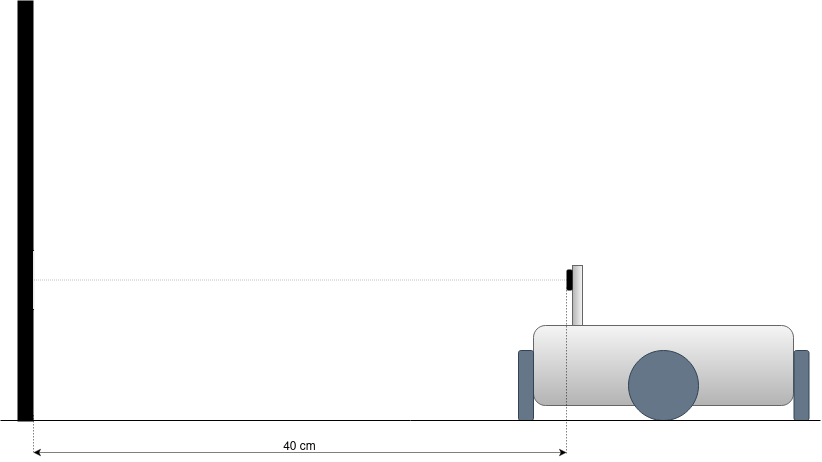
\includegraphics[width=1.0\linewidth]{images/robot_medicion_qr.png}
   \caption{Representación de la obtención de parámetros para calibrar la cámara}
   \label{fig:robot_medicion_qr}
\end{figure}

El objetivo de esta calibración es encontrar la longitud focal, la cual es una constante que representa la distancia desde el centro del objetivo (código QR) hasta el sensor de la cámara y se calcula de la siguiente manera:

\begin{equation}
   Longitud\ focal = \frac{Ancho\ de\ la\ imagen\times Distancia\ Real}{Dimensi\acute{o}n\ real\ del\ c\acute{o}digo\ QR}
   \label{ec:logitud_focal}
\end{equation}

Donde:
\begin{itemize}
   \item El ancho de la imagen se representa en la cantidad de pixeles
   \item La distancia real es entre el código QR y la cámara
   \item La dimensión real del código QR es el ancho del código en la realidad
\end{itemize}

Una vez obtenido este parámetro lo vamos a utilizar para siempre comparar la dimensión en píxeles del código QR en la imagen con el código QR en sí, y de esa manera obtener la distancia que existe hacia el objeto con la fórmula:

\begin{equation}
   Distancia = \frac{Dimensi\acute{o}n\ real\ del\ c\acute{o}digo\ QR \times Longitud\ focal}{Ancho\ del\ QR\ en\ la\ imagen}
   \label{ec:distancia_qr}
\end{equation}

Por supuesto que esto se aplica únicamente cuando en la fotografía se logra identificar un código QR, si durante el procesamiento de la imagen esto no sucede, no se va a poder determinar la distancia. Realizando varias pruebas se logró determinar que sí la cámara se encuentra entre los 50cm y 60cm del objetivo, el código QR es identificable en la imagen, una distancia mayor al rango descrito ya se considera fuera del rango de la distancia focal.

A partir del posicionamiento del robot se obtuvo la siguiente imagen, la cual se usó de referencia para medir la distancia en todas las demás fotografías.
\begin{figure}[H]
   \centering
   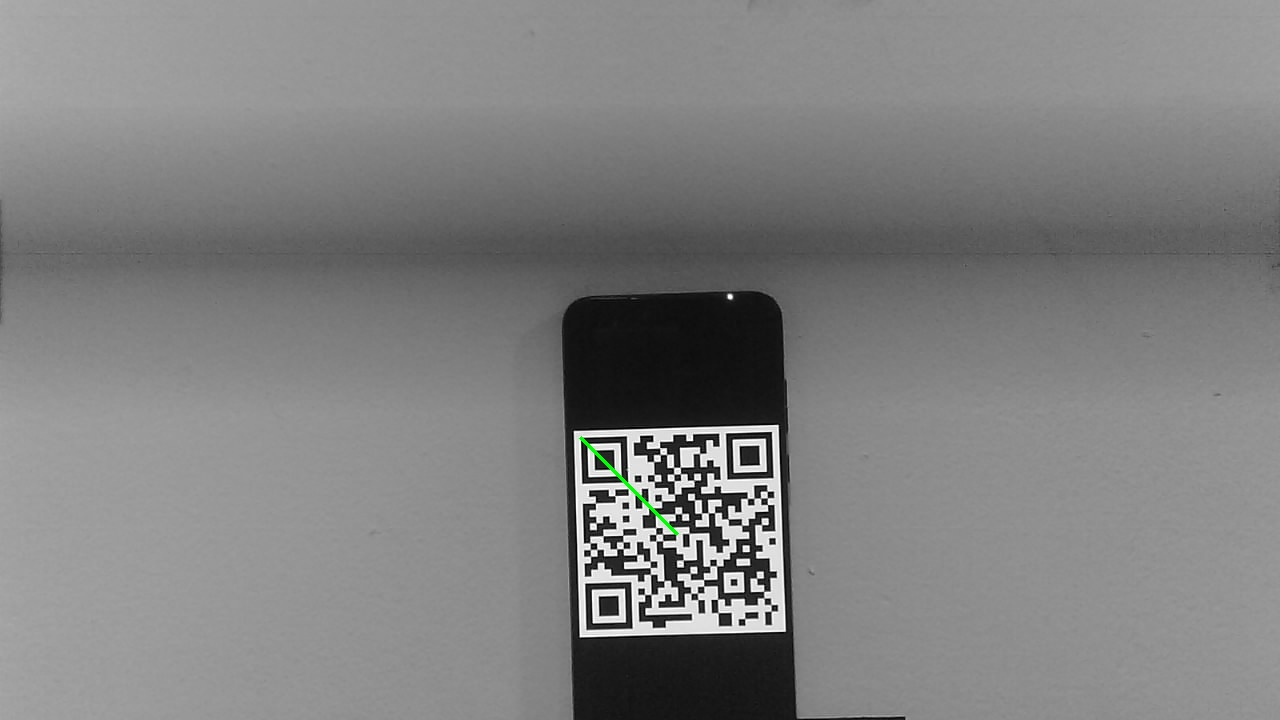
\includegraphics[width=0.8\linewidth]{images/img_centro.jpg}
   \caption{Imagen de referencia obtenida por el robot}
   \label{fig:img_centro}
\end{figure}

Después ya se incorporó toda la lógica al traslado del robot y se reportaron los resultados en movimiento.

\begin{figure}[H]
   \centering
   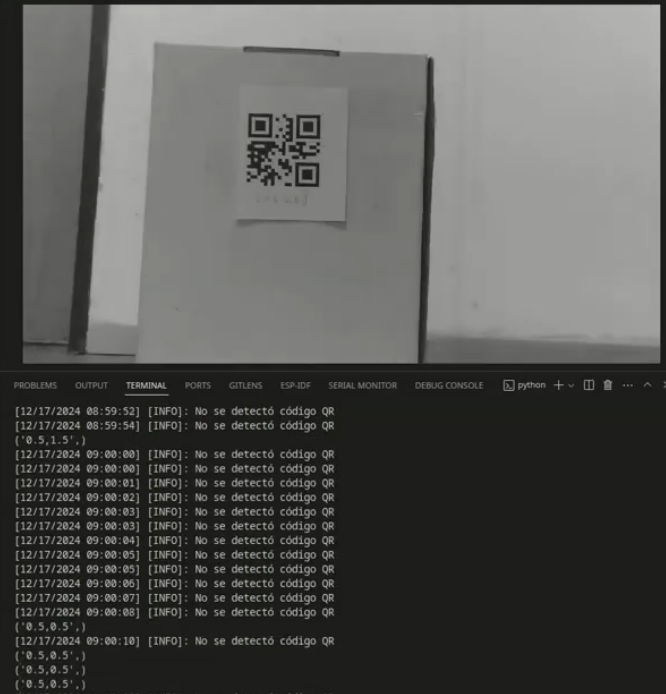
\includegraphics[width=0.7\linewidth]{images/qr.png}
   \caption{Imagen obtenida por el robot en movimiento}
   \label{fig:qr}
\end{figure}